%%%%%%%%%%%%%%%%%%%%%%%%%%%%%%%%%%%%%%%%%%%%%%%%%%%%%%%%%%%%%%%%%
% Tese de Doutorado / Dept Fisica, CFM, UFSC                    %
% Andre@UFSC - 2014                                             %
%%%%%%%%%%%%%%%%%%%%%%%%%%%%%%%%%%%%%%%%%%%%%%%%%%%%%%%%%%%%%%%%%

%:::::::::::::::::::::::::::::::::::::::::::::::::::::::::::::::%
%                                                               %
%                          Capítulo 4                           %
%                                                               %
%:::::::::::::::::::::::::::::::::::::::::::::::::::::::::::::::%

%***************************************************************%
%                                                               %
%                   Morfologia de galáxias                      %
%                                                               %
%***************************************************************%

\chapter{Morfologia de galáxias}
\label{sec:morph}

A descoberta das formas das galáxias, e a sua separação em classes segundo a sua
morfologia, somente se tornou uma ciência séria quando {\em surveys}
fotográficos extensos começaram a ser realizados \citep{Sandage1975}. Pode-se
considerar o ano de 1845 como um marco inicial no estudo da forma das galáxias,
quando Lord Rosse, observando com o telescópio refletor de 72 polegadas no
Castelo de Birr, descobriu estruturas espirais em M51 (Galáxia do Redemoinho, no
catálogo de Messier). À época, pouco se sabia sobre a natureza das ``nebulosas
espirais'' e os esquemas de classificação eram puramente descritivos como o de
\citet{Wolf1908}, mostrado na Figura \ref{fig:WolfEarlyClass}.
\citet{Knox-Shaw1915}, entre outros, chamou a atenção para nebulosas sem braços
espirais, que viriam a ser chamadas mais tarde de elípticas.
\citet{Curtis1918} foi o primeiro a identificar espirais com barra.
Em meados de 1940 já se havia descoberto a maioria dos tipos mais comuns das
``nebulosas extragaláticas'', termo que já começava a cair em desuso em favor do
nome mais glamouroso, segundo o próprio \citet{hubble1936}: ``galáxias''.

\begin{figure}
	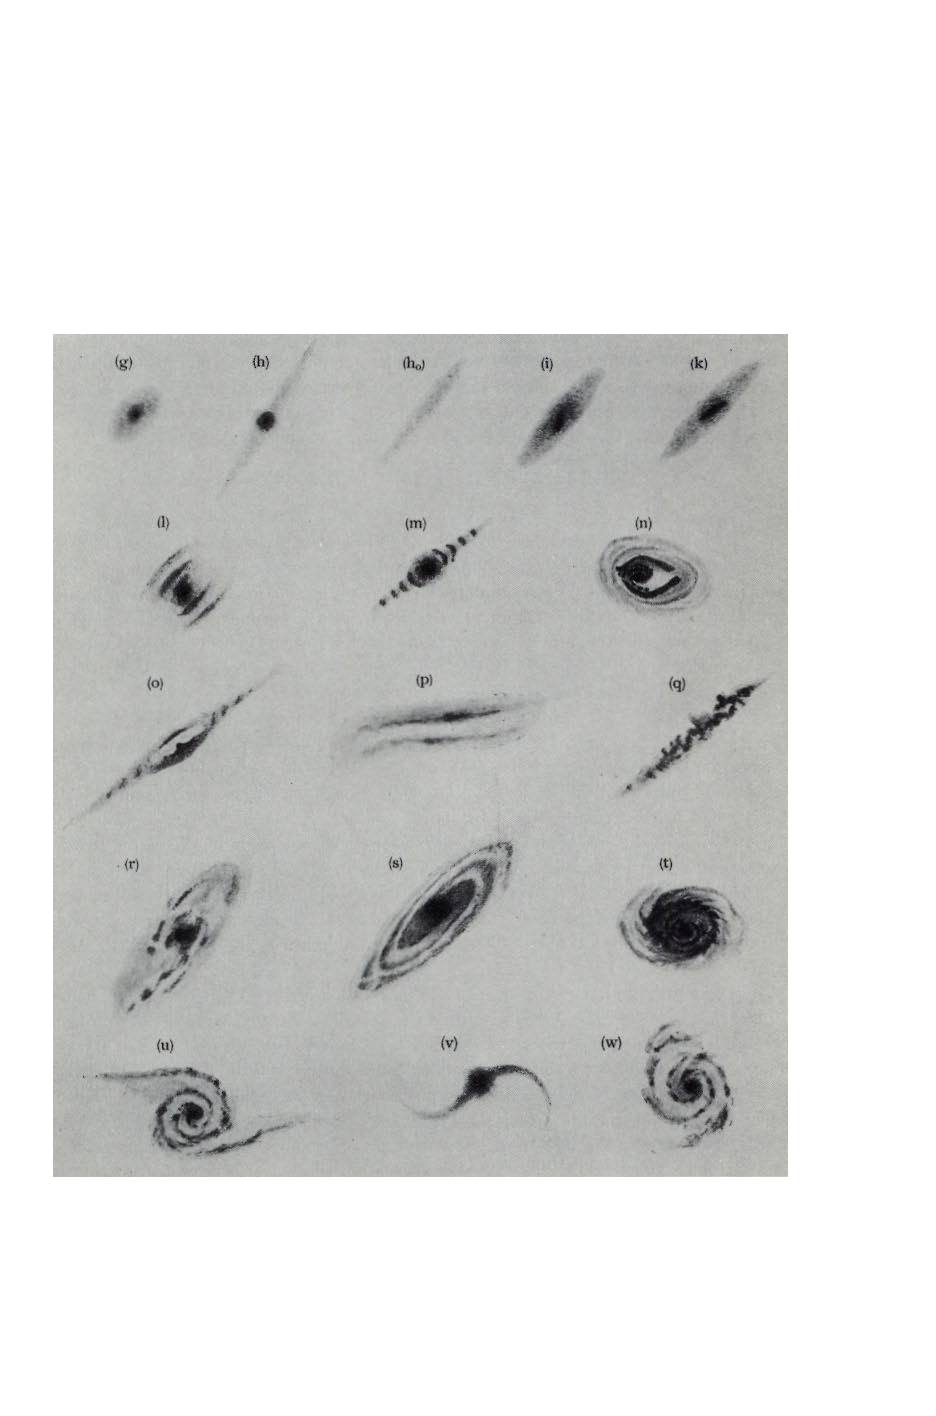
\includegraphics[width=0.7\textwidth]{figuras/WolfEarlyClass}
	\caption[Classificação de Wolf.]
	{Sistema de classificação descritivo de nebulosas por \citet{Wolf1908},
	apresentava também nebulosas galáticas (na primeira linha, que foi removida).
	Reproduzido de \citet{Sandage1975}.}
	\label{fig:WolfEarlyClass}
\end{figure}


%***************************************************************%
%                                                               %
%                   Classificação de Hubble                     %
%                                                               %
%***************************************************************%

\section{Classificação de Hubble}

O primeiro sistema amplamente utilizado de classificação de galáxias segundo a
sua morfologia foi o de \citet{Hubble1926}. Neste sistema, as galáxias são
separadas nas classes elíptica, espiral, espiral com barra e irregular. As
elípticas são classificadas segundo o seu formato, desde esférico até mais
alongado. As espirais são classificadas conforme o tamanho relativo do bojo e as
características dos braços (quantidade, grau de espiralamento e granularidade).
A forma final de classificação de Hubble é frequentemente ilustrada pelo
``diagrama diapasão'', apresentado na Figura \ref{fig:HubbleSequence}, do
clássico {\em The Realm of the Nebulae} de \citet{hubble1936}, e atualizado
(incluindo a classe S0 na intersecção dos ramos das espirais) por
\citet{Sandage1975}.

\begin{figure}
	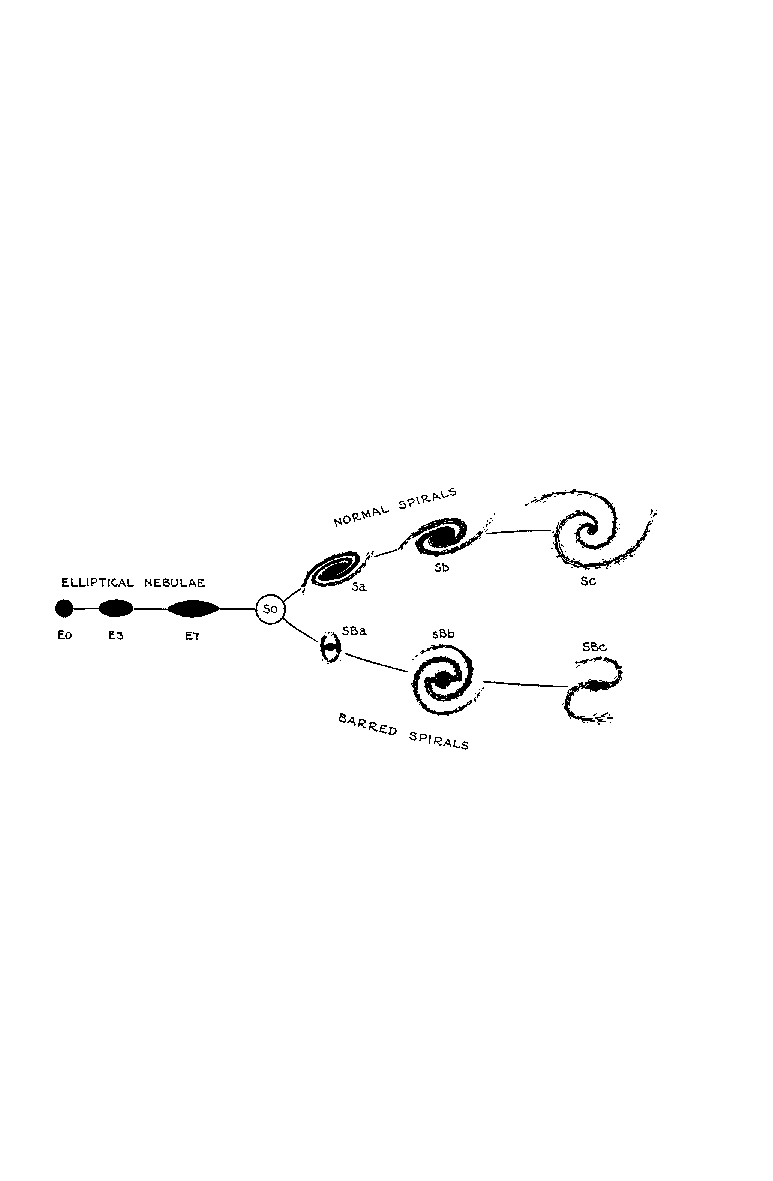
\includegraphics[width=1.0\textwidth]{figuras/HubbleSequence}
	\caption[Classificação de Hubble.]
	{Sistema de classificação de \citet{hubble1936}, também conhecido como
	``diagrama diapasão de Hubble''. Foi atualizado por
	\citet{Sandage1975} para incluir a classe S0 na intersecção dos
	ramos das espirais.}
	\label{fig:HubbleSequence}
\end{figure}

O sistema de Hubble parece ser mais do que um simples ``catálogo botânico'' de
galáxias. Muitas das propriedades observadas das galáxias, como índices de cor,
tipo espectral e densidade de hidrogênio gasoso, variam sistematicamente na
sequência de formas. De algum modo, parece haver algo de fundamental escondido
nesta classificação baseada apenas na forma, que talvez indique uma relação com
as condições iniciais e subsequente evolução temporal das galáxias
\citep{Sandage1975}. Estas correlações fizeram com que, durante muito tempo, a
sequência de Hubble fosse considerada uma sequência evolutiva, onde as galáxias
eram inicialmente elípticas, passavam a ser lenticulares e depois espirais. Isto
sobrevive até hoje na nomenclatura ``{\em early type}'' (tipo jovem) para
elípticas e lenticulares, e ``{\em late type}'' (tipo tardio) para espirais e
irregulares. Entretanto, \citet{Hubble1927} enfatizou desde o início que a
classificação era puramente empírica, e que interpretações de natureza evolutiva
deveriam ser tomadas com cautela.


%***************************************************************%
%                                                               %
%                   Componentes estruturais                     %
%                                                               %
%***************************************************************%

\section{Componentes estruturais}

Os sistemas de classificação descritos na seção anterior são baseados em
inspeção visual, com natureza evidentemente qualitativa. Levando tal forma de
classificação a um extremo, como o projeto {\em GalaxyZoo} \citep{Lintott2008,
Willett2013}, chega-se a conclusões estatísticas, mas ainda não se obtém medidas
quantitativas de objetos individuais. Para descrever mais precisamente a
estrutura de uma galáxia, normalmente é necessário decompô-la em sub-estruturas.
Estas sub-estruturas são em geral modeladas como funções analíticas, as quais
permitem derivar medidas quantitativas. De forma simplificada, podemos
considerar que galáxias são compostas de duas componentes principais: bojo e
disco. Os próprios discos podem conter barras, braços espirais, anéis e halos,
para citar algumas sub-componentes mais comuns.


\subsection{Bojos e discos}
\label{sec:morph:comp:bd}

Do ponto de vista fotométrico (medindo o perfil de brilho superficial), galáxias
lenticulares (S0) e espirais {\em early type} (Sa-Sb) podem ser bem descritas
como uma combinação de duas componentes: um bojo e um disco. Neste modelo, o
disco é delgado enquanto o bojo é quase esférico (embora haja casos em que ele
seja um elipsóide triaxial), ambos observados projetados no plano do céu.

Levando em consideração apenas o perfil de brilho superficial, a separação em
componentes baseado no aspecto visual parecer arbitrária. Afinal, pode-se
inventar algum modelo empírico onde uma só componente descreva as imagens
observadas tão bem quanto a soma de um bojo e um disco. Porém, estas componentes
parecem ter outras propriedades distintas, como índices de cores, conteúdo de
gás e poeira, cinemática e populações estelares, o que confere uma certa
confiança no conjunto de componentes escolhido.

\citet{King1966} descreve um modelo derivado para aglomerados globulares,
assumindo velocidades estelares isotérmicas e isotrópicas. Muito embora este
modelo tenha motivações físicas, não possui uma forma funcional simples. Leis
como as de Hubble-Reynolds \citep[equação 2.55]{Binney2011} e
\citet{deVaucouleurs1948, deVaucouleurs1977}, mesmo sendo puramente empíricas,
descrevem bem bojos de galáxias. Suas formas funcionais são:
\begin{equation*}
I(r) &= \frac{I_0}{\left[1 + \left(\sfrac{r}{r_H}\right)^2\right]}
&\text{(Hubble-Reynolds)} \\
I(r) &= I_e \exp \left\{-7,67 \left[\left(\frac{r}{r_e}\right)^{1/4} -
1\right]\right\} &\text{(de Vaucouleurs)}
\end{equation*}

Os termos $r_e$ e $r_H$ são os parâmetros de escala radial, $I_0$ é o
brilho para $r\!=\!0$ na lei de Hubble-Reynolds e $I_e$ é o brilho para $r=r_e$
na lei de de Vaucouleurs. Estas formas funcionais se ajustam bem à maioria dos
bojos e galáxias elípticas. Para sistemas que não são esféricos, deve-se ainda
introduzir uma elipticidade e uma orientação. Adicionalmente, a elipticidade e a
orientação podem variar com o raio.

Discos, por outro lado, são facilmente modelados como um perfil exponencial
\citep{Freeman1970} dado por
\begin{equation*}
I(r) = I_0 \exp\left(\frac{r}{h}\right),
\end{equation*}
com $h$ sendo o parâmetro de escala radial, e $I_0$ o brilho em $r\!=\!0$.

\begin{figure}
	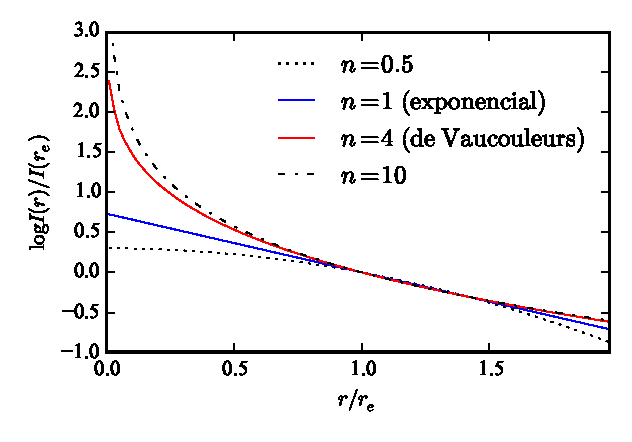
\includegraphics{figuras/morphModels}
	\caption[Perfis empíricos de Sérsic.]
	{Perfis empíricos de Sérsic. O índice $n$ controla a concentração do perfil.
	Com $n\!=\!1$ obtém-se um perfil exponencial (azul), e com $n\!=\!4$ um perfil
	de de Vaucoulerus (vermelho). Outros valores de $n$ são mostrados em
	linhas descontínuas.}
	\label{fig:MorphLaws}
\end{figure}

\citet{Sersic1963} mostra que os perfis de de Vaucouleurs e exponencial podem
ser tomados como casos particulares da equação
\begin{equation*}
I(r) = I_e \exp \left\{- b_n \left[ \left( \frac{a}{r_e} \right)^{1/n}
- 1 \right] \right\},
\end{equation*}
que ficou conhecida como ``lei de Sérsic''. Aqui, o parâmetro $n$ é o índice de
concentração, também chamado de ``índice de Sérsic'', que pode variar
continuamente. A Figura \ref{fig:MorphLaws} mostra alguns exemplos. Com
$n\!=\!1$ obtém-se uma lei exponencial (linha azul), e com $n\!=\!4$ a lei de de
Vaucouleurs (linha vermelha). A maioria dos bojos de espriais e galáxias
elípticas podem ter seus perfis de brilho ajustados com índices de Sérsic na
faixa de $1 < n < 10$. Valores maiores de $n$ mudam muito pouco a forma da
curva. O parâmetro $b_n$ está definido em função de $n$, ver a seção 6.1.5 de
\citet{Erwin2015}.

É preciso ter em mente que estas leis são empíricas, e dependem do bom senso de
escolher o perfil (ou conjunto de perfis) certo para a galáxia em questão.
Tentar ajustar um modelo inapropriado a uma galáxia pode levar a conclusões
equivocadas, embora o ajuste possa parecer bem sucedido.


\subsection{Dependência dos modelos com o comprimento de onda}
\label{sec:morph:comp:depLambda}

Tudo o que se discutiu sobre classificação de galáxias quanto a sua forma, até
agora, levou em conta imagens feitas no banda óptica do espectro. Basta olhar
umas poucas galáxias em infravermelho ou ultravioleta para verificar que a forma
de uma galáxia pode mudar dramaticamente dependendo do comprimento de onda em
que se observa. Bojos normalmente desaparecem em ultravioleta por possuírem
poucas estrelas jovens. Já em infravermelho, os bojos tendem a dominar, e discos
podem ter uma forma bastante diferente por conta da menor profundidade óptica
das estruturas de poeira. Claramente há uma dependência da morfologia das
galáxias com o comprimento de onda.

\begin{figure}
	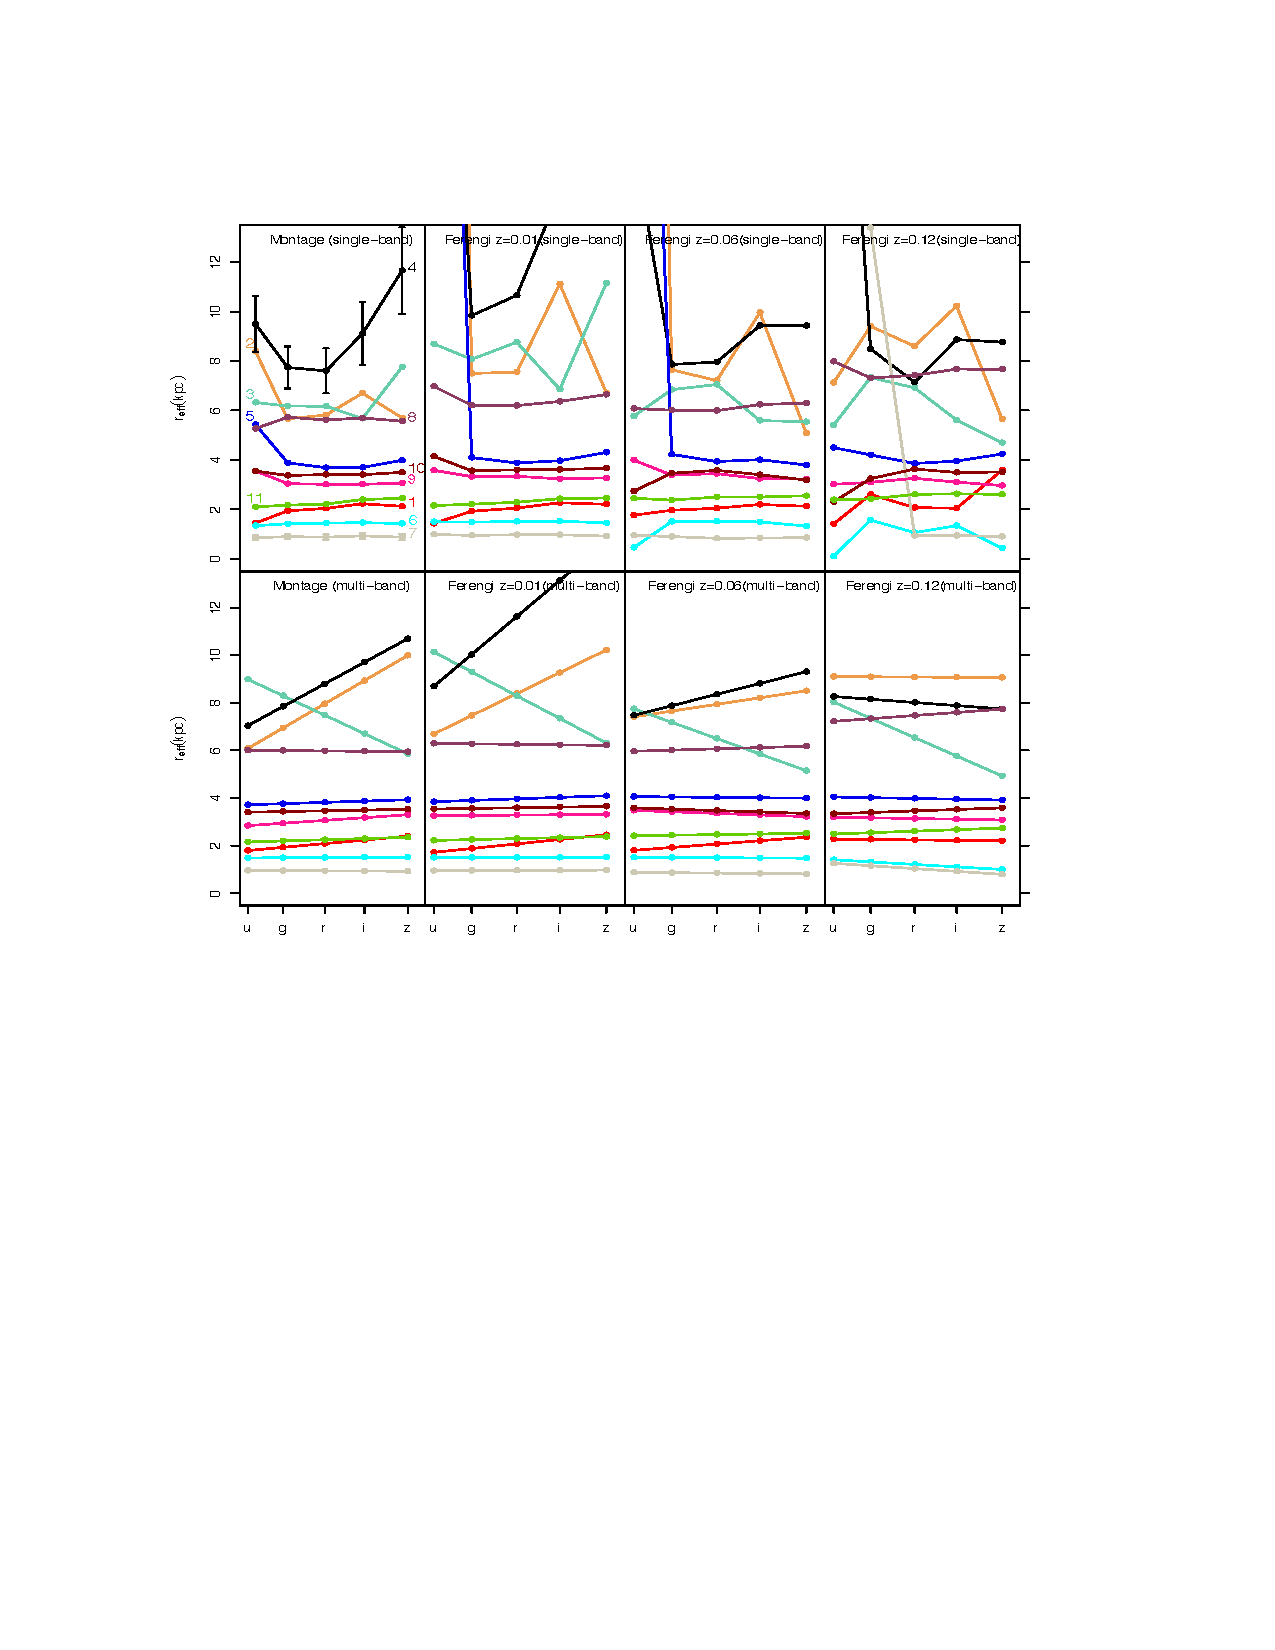
\includegraphics{figuras/vika-properties}
	\caption[Ajuste morfológico de bandas fotométricas] {Ajuste
	morfológico de 11 galáxias, utilizando as bandas fotométricas do
	SDSS. Os gráficos mostram o raio efetivo ($r_e$ neste trabalho) ajustado
	livremente a cada banda (painéis superiores), e com uma dependência linear em
	comprimento de onda (painéis inferiores). À esquerda estão os ajustes com as
	imagens originais, as colunas seguintes são para imagens com {\em redshift}
	artificiais. Retirado de \citet{Vika2013}.}
	\label{fig:propertiesVika}
\end{figure}

\citet{Kelvin2012} utilizou imagens de galáxias do projeto GAMA
\citep{Driver2009} em 9 bandas espectrais, do óptico \citep[bandas $ugriz$ do
DR7]{Abazajian2009} ao infravermelho \citep[bandas $YJHK$ do
UKIDSS]{Lawrence2007}, para ajustar perfis de Sérsic a $>\!160.000$ galáxias,
encontrando gradientes leves no índice de Sérsic em função do comprimento de
onda. Os ajustes para cada comprimento de onda foram feitos individualmente. O
projeto MegaMorph \citep{Haussler2013} faz o mesmo de uma forma um pouco mais
refinada. Utilizando as bandas fotométricas do SDSS, eles ajustam a variação dos
parâmetros morfológicos através de um polinômio \citep[Figura
\ref{fig:propertiesVika}]{Vika2013}. Todos os comprimentos de onda são ajustados
de uma vez. Aí se pode ver que em grande escala (em comprimento de onda), há
galáxias com um comportamento linear (ou até razoavelmente constante) em $r_e$.
Nestes casos, utilizar um modelo linear em função do comprimento de onda,
segundo os autores, melhora a qualidade do ajuste.

Além de efeitos causados pelo método de ajuste, como má escolha do modelo,
mudança no sinal-ruído nas várias bandas espectrais, ou mínimos locais, parece haver
motivos reais para levar a sério a variação dos parâmetros morfológicos.
Populações estelares diferentes emitem mais intensamente em comprimentos de onda
distintos, com populações mais jovens dominando em comprimentos de onda menores.
Isto parece causar um leve gradiente no índice de Sérsic em galáxias {\em early
type} \citep{LaBarbera2009}. Poeira parece afetar a medida do tamanho
e forma de discos \citep{Mollenhoff2006}. O conteúdo e a distribuição de poeira e pode
variar significativamente de galáxia a galáxia, dificultando uma conclusão
global sobre o seu efeito nos parâmetros morfológicos.

\begin{figure}
	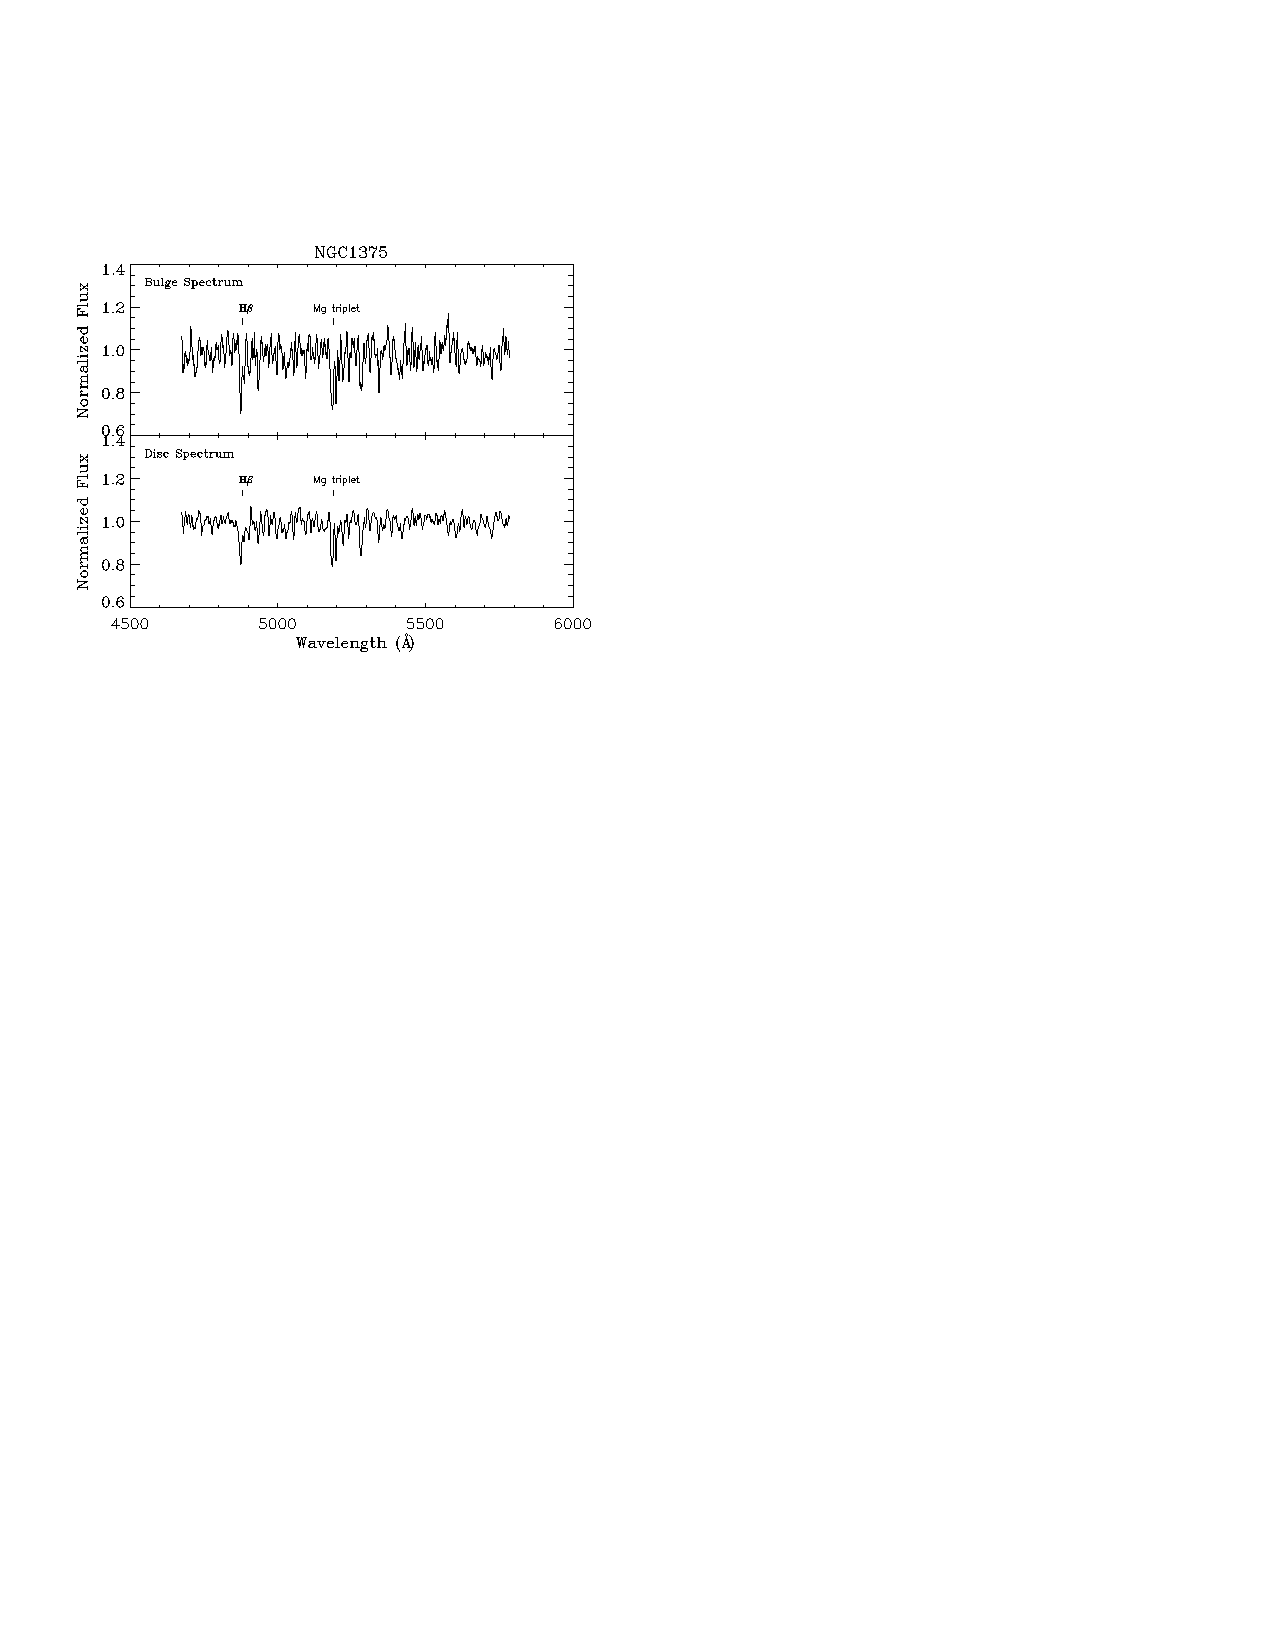
\includegraphics{figuras/johnston-spectra}
	\caption[Espectros das componentes morfológicas.] {Espectros unidimensionais de
	bojo (acima) e disco (abaixo) de NGC 1375. É possível reconhecer a
	linha espectral \Hbeta e o tripleto de magnésio, em absorção. Retirado de
	\citet{Johnston2012}.}
	\label{fig:spectraJohnston}
\end{figure}

\begin{figure}
	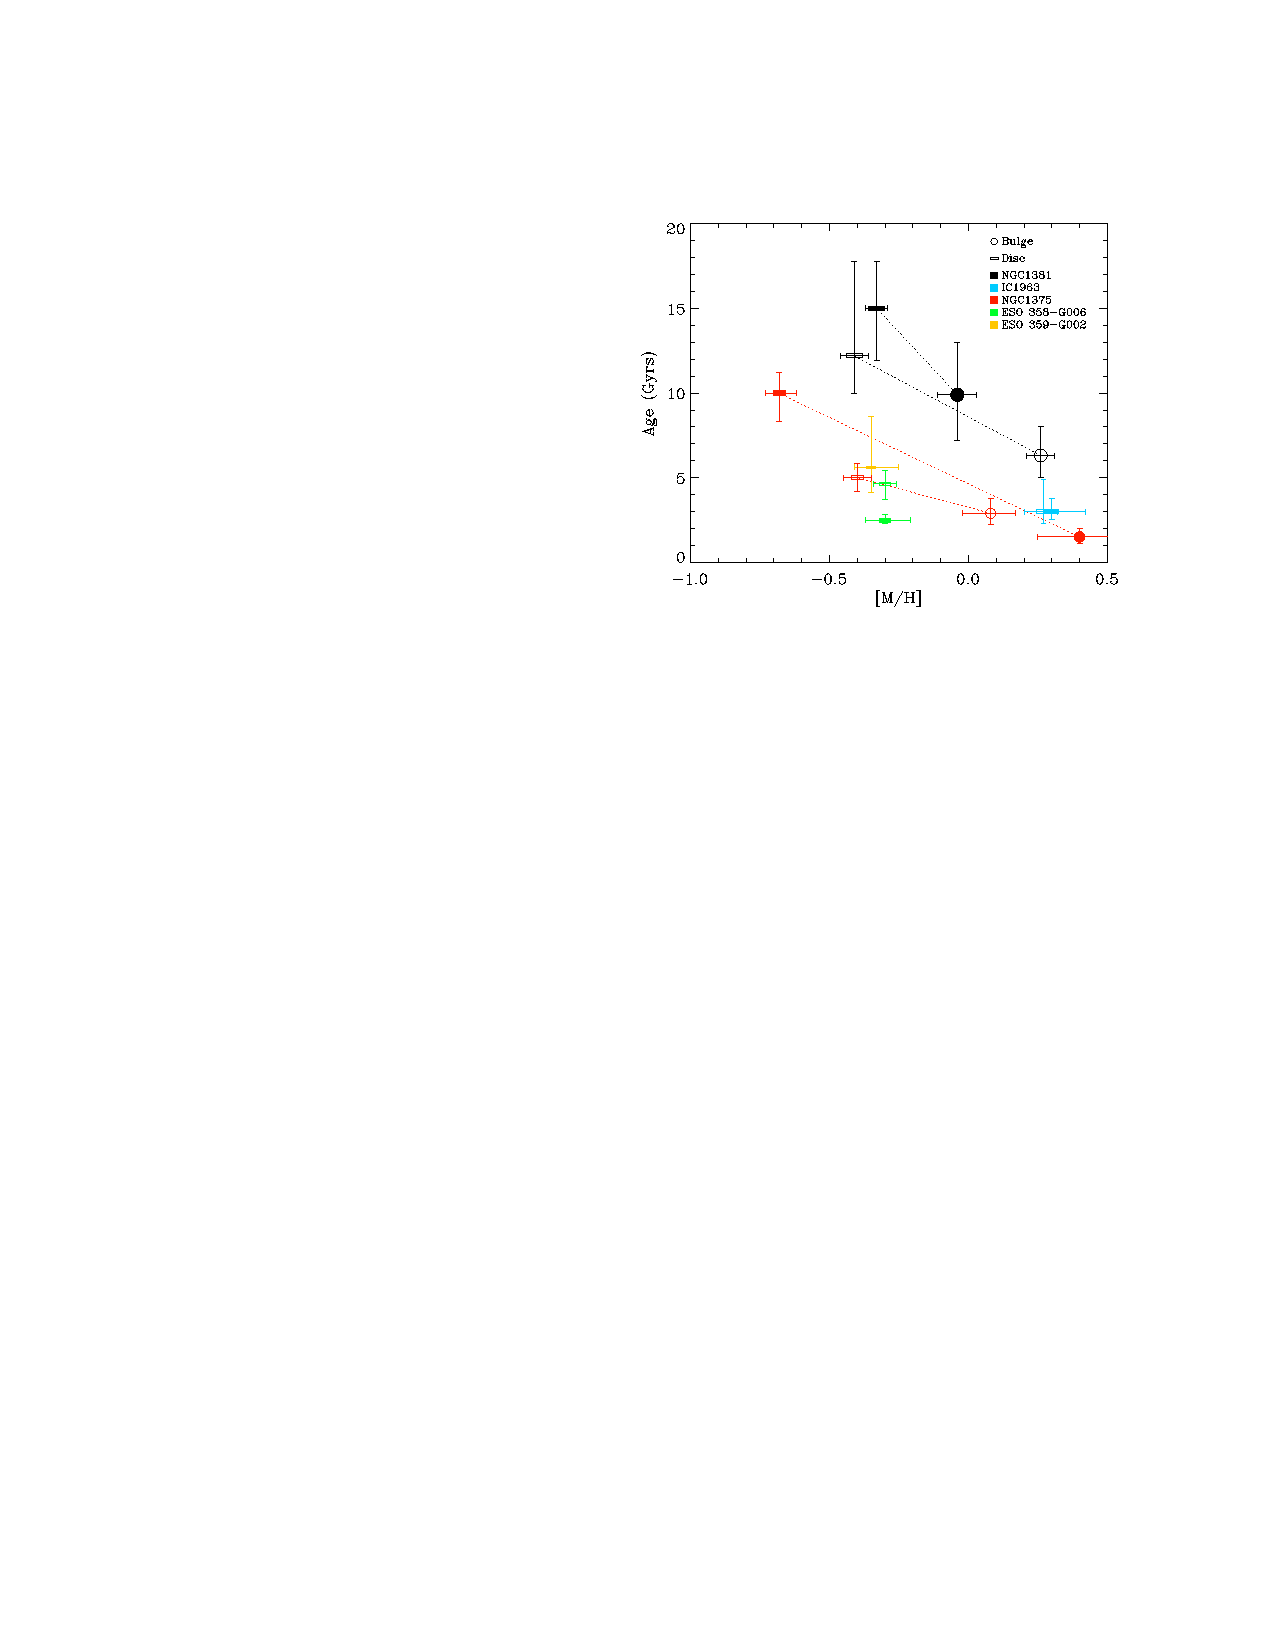
\includegraphics{figuras/johnston-pop}
	\caption[Idade e metalicidade de bojos e discos de galáxias S0.] {Idade (eixo
	vertical) e metalicidade (eixo horizontal) estelares de bojos (marcadores
	redondos) e discos (marcadores retangulares) de uma amostra de galáxias S0
	observadas com espectrógrafo de fenda longa. As linhas pontilhadas ligam
	componentes de uma mesma galáxia. Retirado de \citet{Johnston2012}.}
	\label{fig:populationJohnston}
\end{figure}

\citet{Johnston2012} obtiveram espectros de fenda longa de galáxias lenticulares
(S0), gerando assim perfis de brilho das galáxias para cada comprimento de onda.
Ajustando um perfil de de Vaucouleurs e um exponencial ao perfil de brilho de
cada uma das galáxias (em ambos os lados), eles obtém os espectros separados de
cada um dos seus dois componentes morfológicos, como mostrado na Figura
\ref{fig:spectraJohnston}. Com os espectros, pode-se tentar entender que
populações estelares compõe o bojo e o disco destes galáxias. Os autores estimam
a idade e a mtelicidade estelar das componentes utilizando a intensidade da
linha \Hbeta e do tripleto de magnésio, comparando com uma grade de modelos
sintéticos de populações estelares. A conclusão que chegam é que os bojos são
sistematicamente mais jovens e mais metálicos do que os discos (Figura
\ref{fig:populationJohnston}). Inspirado neste estudo, o Capítulo
\ref{sec:Decomp} descreve a decomposição de espectros de galáxias em espectros
de bojos e discos, mas utilizando cubos de dados do CALIFA.


\subsection{Ajuste de modelos}
\label{sec:morph:comp:ajuste}

Utiliza-se geralmente algoritmos de minimização para encontrar os modelos que
melhor ajustam o perfil de brilho de uma galáxia. A abordagem usual é baseada no
princípio de máxima verossimilhança ($\mathcal{L}$). Se a estatística das
medidas é gaussiana (que é aproximadamente verdade na maioria das imagens
astronômicas relevantes ao ajuste de modelos), o logarítmo da verossimilhança se
assemelha à familiar soma de $\chi^2$\citep[seção 4.1.2]{Erwin2015}. Isto
significa que o problema passa a ser a minimização da equação
\begin{equation*}
-2\ln\mathcal{L} = \chi^2 = \sum_i^N \frac{\left(d_i -
m_i\right)^2}{\sigma_i^2},
\end{equation*}
onde $d_i$ é o valor medido, $m_i$ é o valor do modelo, e $\sigma_i$ é o erro
gaussiano na medida. O modo como se procura o mínimo $\chi^2$ vai depender de
como se aborda o problema.

\begin{figure}
	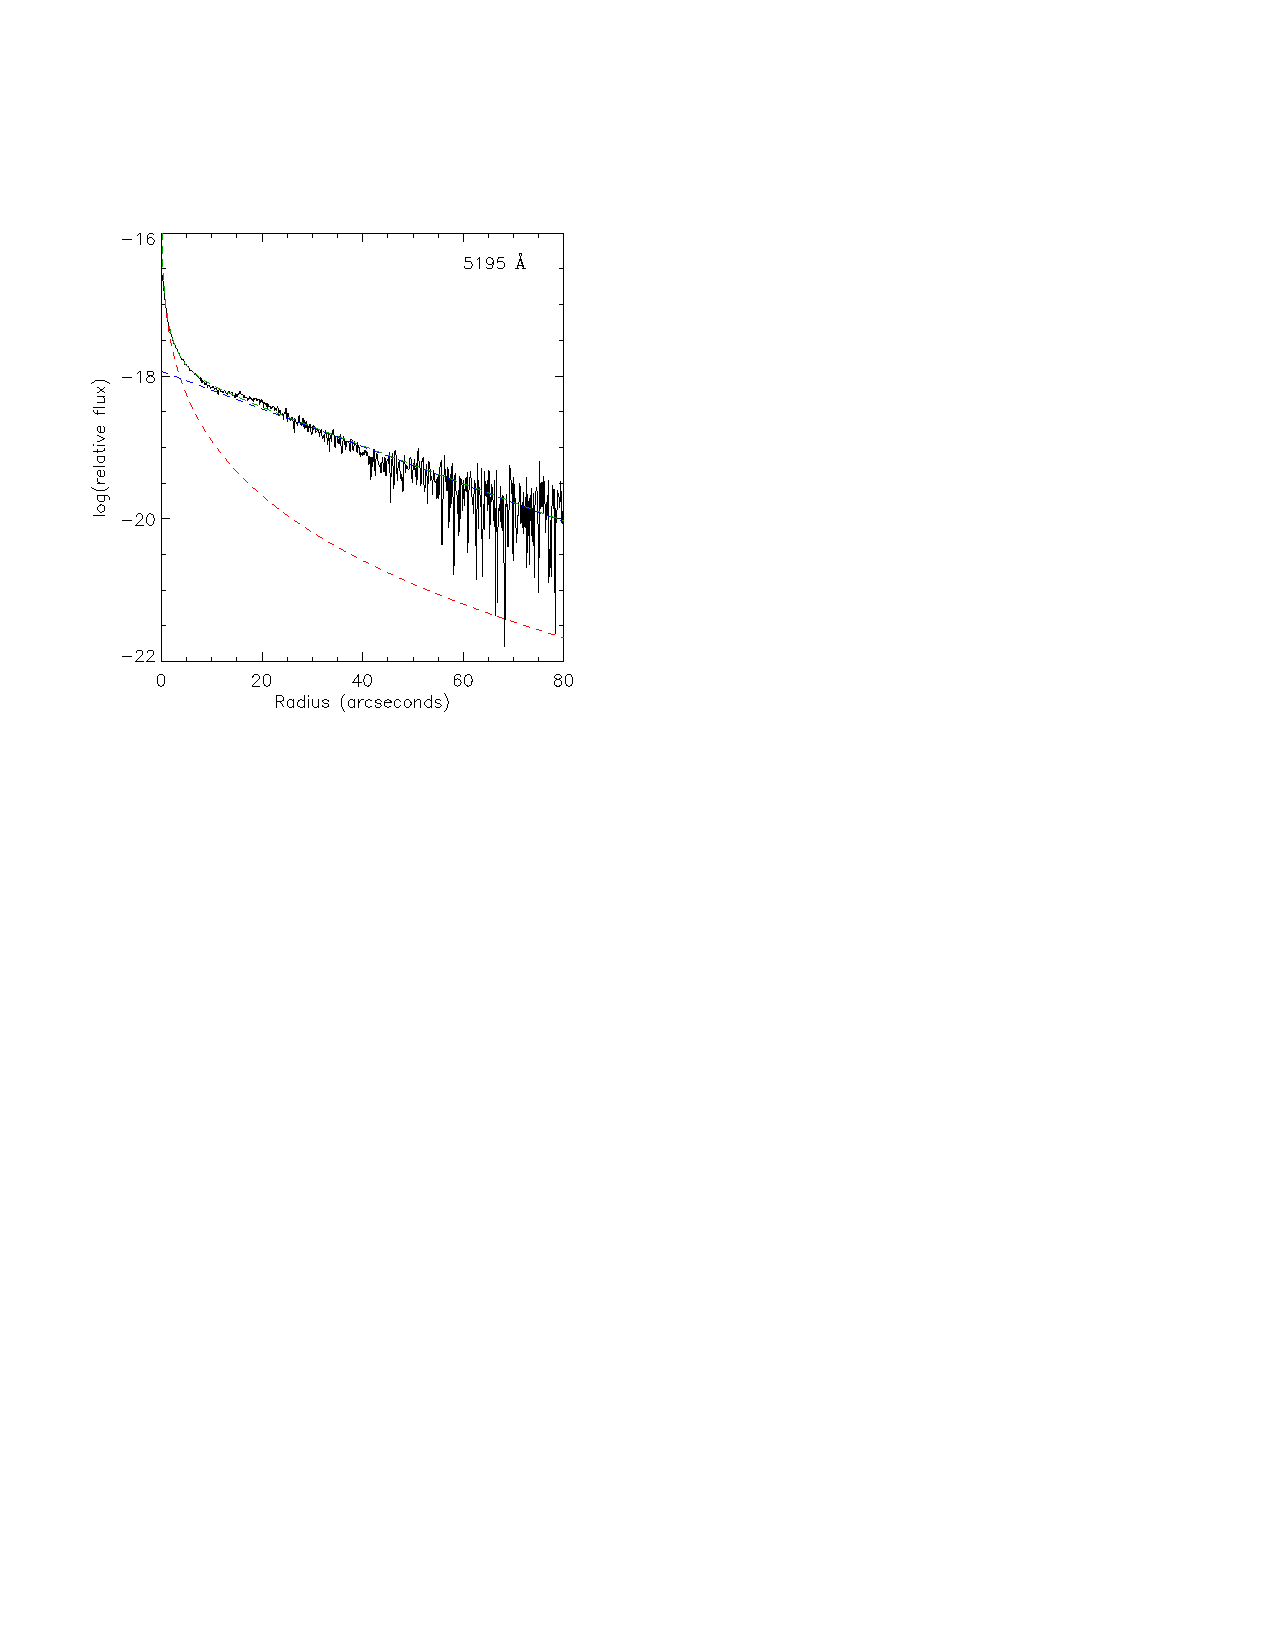
\includegraphics{figuras/johnston-decomp}
	\caption[Ajuste morfológico em uma dimensão] {Ajuste morfológico
	em uma dimensão, utilizando modelos de bojo e disco. A linha preta mostra o
	perfil de brilho da galáxia NGC 1375 em $5195\,\angstrom$, obtido através de
	espectroscopia de fenda longa. Em azul um perfil exponencial e em vermelho um
	perfil de De Vaucouleurs (Sérsic com $n=4$), que somados são o melhor ajuste,
	em verde. Retirado de \citet{Johnston2012}.}
	\label{fig:decompJohnston}
\end{figure}

\begin{figure}
	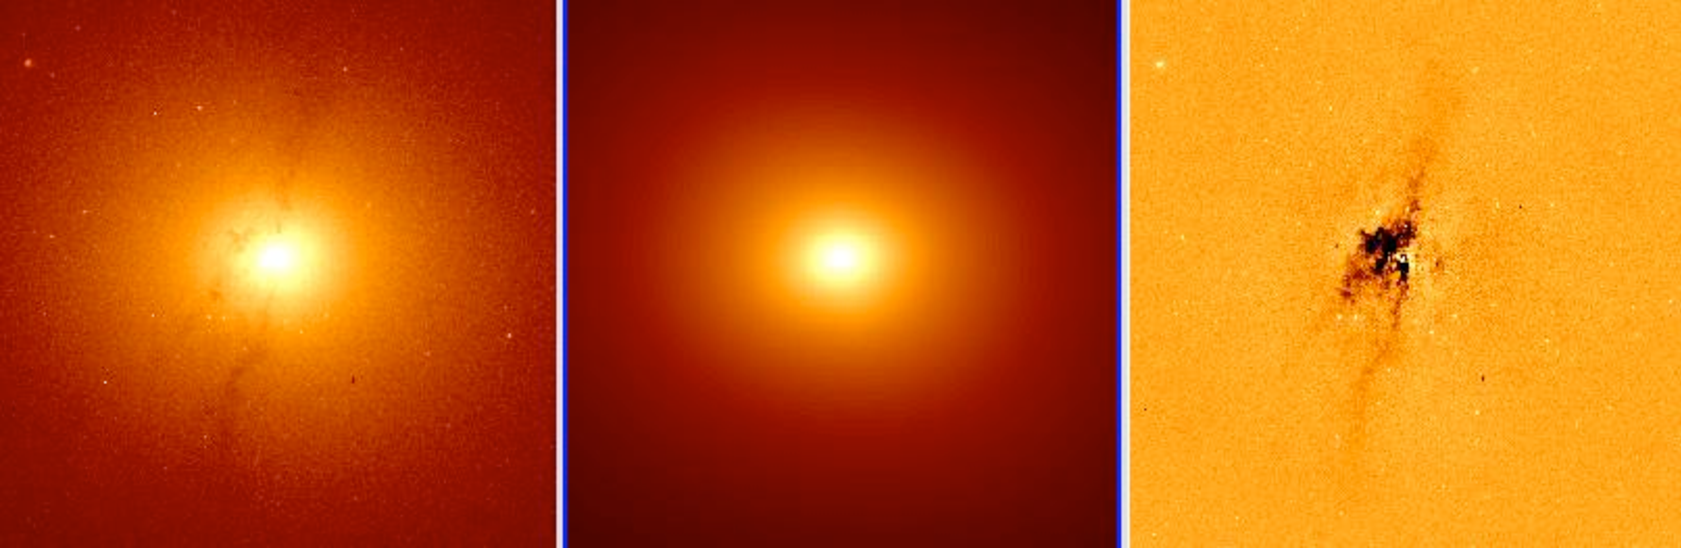
\includegraphics[width=1.0\textwidth]{figuras/galfit-decomp}
	\caption[Ajuste morfológico em duas dimensões] {\TODO Ajuste morfológico
	em duas dimensões, feito de alguma forma com GALFIT \citep{Peng2002}. Procurar
	uma figura melhor.}
	\label{fig:decompGalfit}
\end{figure}

A Figura \ref{fig:decompJohnston} mostra um exemplo de ajuste de bojo e disco em
um perfil de brilho unidimensional. Pode-se fazer o ajuste diretamente na
imagem, em duas dimensões (Figura \ref{fig:decompGalfit}), utilizando modelos
com perfis elipsoidais. Independente da escolha do modelo, há um aspecto
importante do ajuste da morfologia que foi negligenciado até agora: efeitos
instrumentais e atmosféricos. Estes efeitos são representados pela figura da PSF
({\em Point Spread Function}), tratada em detalhes no Capítulo \ref{sec:psf}. A
grosso modo, levar em conta a PSF significa considerar que a luz que atinge
determinada posição no detector não é proveniente apenas de uma região pontual
no céu, e sim de uma região extensa que depende dos instrumentos e da tubulência
atmosférica. Efetivamente, objetos pontuais tornam-se ``borrões'' na imagem
observada.

Pode-se evitar tocar neste ponto quando se faz o ajuste em uma dimensão.
Se as dimensões da PSF forem muito menores do que as da galáxia, e esta tiver
uma imagem suave, a forma da galáxia muda muito pouco devido à PSF, exceto
exatamente sobre o núcleo. Isto é especialmente problemático em {\em early
types}, onde um perfil de Sérsic pode gerar um pico de várias ordens de
magnitude, concentrado em uns poucos em {\em pixels}. A forma mais simples de se
escapar da PSF, em uma dimensão, é ``varrê-la para baixo do tapete'', isto é,
não tentar ajustar pontos muito próximos ao núcleo (mascarando alguns segundos
de arco, dependendo do tamanho da PSF). O ajuste de um perfil de Sérsic pode
ficar comprometido em casos onde a PSF é muito grande e se descarta uma fração
considerável do bojo.

Em duas dimensões o mais adequado é adotar a PSF como parte do problema. Uma boa
caracterização da PSF é crucial para se obter resultados satisfatórios no
ajuste. Mas, trabalhar com a PSF traz um custo computacional enorme, uma vez que
é preciso efetuar um cálculo de convolução (ver Seção \ref{sec:psf:teoria}) cada
vez que se avalia o modelo para um determinado conjunto de parâmetros. O
problema de minimização, que já é de natureza não-linear para modelos de
componentes de galáxia, tona-se ainda mais complicado.

Diversos algoritmos foram desenvolvidos para tratar do problema de minimização
não-linear. O método Levenberg-Marquardt \citep[daqui em diante
L-M]{Levenberg1944, Marquardt1963}, com sua busca através do gradiente no espaço
de parâmetros, tem a vantagem de ser muito rápido. Mas, sua própria natureza de
gradiente faz com que seja necessário um bom ``chute inicial'', com a
possibilidade de ficar preso em mínimos locais. Pode-se reduzir a chance de ser
pêgo em mínimos locais utilizando algoritmos mais complexos, como o Nelder-Mead
{\em simplex} \citep[daqui em diante N-M]{Nelder1965}. A desvantagem é que
conforme se vai aumentando a complexidade do algoritmo, o tempo necessário para
encontrar o mínimo tende a crescer drasticamente. De qualquer modo, tanto o L-M
quanto o N-M sofrem de um problema comum: é preciso especificar um valor
inicial, e o algoritmo segue um ou mais caminhos até encontrar o mínimo. O
algoritmo de Metropolis \citep{Metropolis1953, Saha1994} adota uma abordagem
Bayesiana, e o problema de minimização se torna análogo a um problema de
mecânica estatística\fixme, onde se vai baixando a temperatura até encontrar o
estado de menor energia. São necessários apenas os limites do espaço de
parâmetros, uma grande vantagem em casos onde não se sabe de antemão o modelo
aproximado. Novamente troca-se velocidade por robustez, este algoritmo é
significativamente mais lento do que L-M e N-M. {\em Differential Evolution}
\citep[daqui em diante DE]{Storn1997} aborda o problema de forma completamente
distinta. Nele, a busca através do espaço de parâmetros é feita com uma
população de modelos. Os modelos sofrem ``mutações'' e ``recombinações'' em cada
iteração, e somente os modelos que se saem melhor são mantidos. Algoritmos desta
natureza são chamados genéticos. Como o algoritmo de Metropolis, apenas são
necessários os limites do espaço de parâmetros. Outra vantagem é que é muito
mais improvável que este algoritmo fique preso num mínimo local do que o L-M, o
N-M ou mesmo o de Metropolis. Tudo isto cobra um grande preço: ele é o algoritmo
mais lento considerado aqui, cerca de duas ordens de magnitude mais lento do que
o L-M.

Existem diversas ferramentas utilizadas em astrofísica que implementam algum
destes algoritmos para fazer o ajuste de modelos em imagens. Vale citar, por
exemplo, GALFIT3 \citep{Peng2010} e GASP2D \citep{MendezAbreu2008} utilizando
L-M, BUDDA \citep{DeSouza2004} utilizando N-M, GIM2D \citep{Simard2002}
utilizando o algoritmo de Metropolis, e
IMFIT\footnote{\url{http://www.mpe.mpg.de/~erwin/code/imfit/index.html}}
\citet{Erwin2015}, que utiliza L-M, N-M ou DE. O programa escolhido para o
presente trabalho foi o IMFIT, em grande parte por ter seu código livre, e
também por ter sido desenvolvido tendo em mente a facilidade de modificação.
Entretanto, como a versão original foi feita em forma de um programa executado
em linha de comando, não é muito prático utilizá-la em seu formato original para
implementar as tarefas deste trabalho.

Foi feita uma versão modificada do IMFIT em forma de biblioteca dinâmica, com um
envelope de código\fixme para ser acessado em Python. Esta biblioteca foi
chamada python-imfit\footnote{\url{https://github.com/streeto/python-imfit}}, e
expõe\fixme praticamente toda a funcionalidade do IMFIT, utilizando {\em arrays}
numéricos do Python. Esta biblioteca é bastante genérica, e pode ser utilizada
para qualquer aplicação de ajuste de imagem. Contudo, o mais importante é que a
manipulação de modelos e o ajuste para múltiplas imagens deixa de ser um
exercício tedioso de organização de {\em shell scripts}\fixme, passando a ser um
programa de computador propriamente dito, com toda a maquinaria do Python a sua
disposição. O programa resultante, que faz a decomposição em bojo e disco em um
cubo de dados do CALIFA, é apresentado no Capítulo \ref{sec:Decomp}.

% End of this chapter
